\section{Clustering}


%\subsection{Grundlagen}


\begin{frame}%1
\frametitle{Grundlagen des Clustering}

\begin{itemize}
\item \hl{Prinzip des Clustering}
\begin{itemize}
\item Häufungspunkt von Objekten im multidimensionalen Raum 
\end{itemize}
\item \hl{Distanzfunktionen}
\begin{itemize}
\item Konstruktion zentraler Punkte 
\item Auswahl repräsentativer Punkte 
\end{itemize}
\item\hl{Clusterverfahren}
\end{itemize}

\end{frame}

%---------------------------------------------------------------------

\begin{frame}%2
\frametitle{Anwendung des Clustering}

\begin{itemize}
\item \hl{Ziel des Clustering} 
\begin{itemize}
\item Identifikation einer endlichen Menge von Kategorien/Klassen
  (\hl{Clustern}) um Daten so zu beschreiben, dass 
\begin{enumerate}[(a)]
\item Objekte im gleichen Cluster möglichst ähnlich und 
\item Objekte aus verschiedenen Clustern möglichst unähnlich zueinander sind
\end{enumerate}

\end{itemize}

\begin{center}
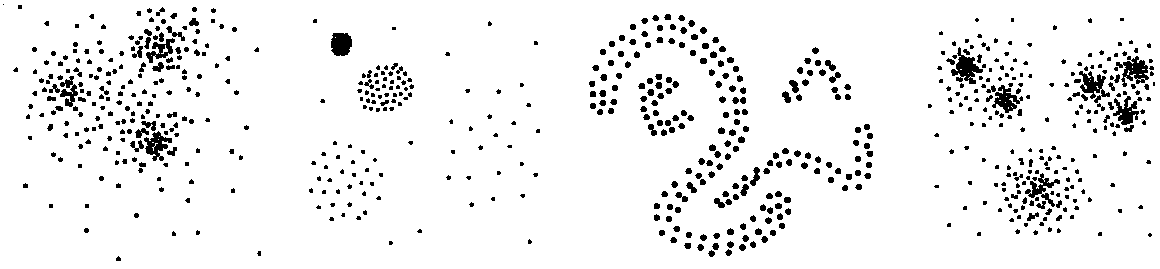
\includegraphics[scale=.4]{fig7/cluster-formen.pdf}
\end{center}

\item \hl{Probleme} 
\begin{itemize}
\item Ähnlichkeitsbegriff 
\item Cluster unterschiedlicher Größe, Form und Dichte
\item Cluster können hierarchisch ineinander verschachtelt sein
\end{itemize}
\end{itemize}
\end{frame}

%---------------------------------------------------------------------

\begin{frame}%3
\frametitle{Anwendungsbeispiele}

\begin{itemize}
\item \hl{Übersicht}
\begin{itemize}
\item  Kundensegmentierung 
\begin{itemize}
\item  Clustering der Kundentransaktionen 
\end{itemize}
\item  Bestimmung von Benutzergruppen auf dem Web 
\begin{itemize}
\item  Clustering der Web-Logs 
\end{itemize}
\item  Strukturierung von großen Mengen von Textdokumenten 
\begin{itemize}
\item  Hierarchisches Clustering von Textdokumenten 
\end{itemize}
\item  Erstellung von thematischen Karten aus Satellitenbildern 
\begin{itemize}
\item  Clustering der aus Rasterbildern gewonnenen Featurevektoren 
\end{itemize}
\end{itemize}
\end{itemize}

\end{frame}


%---------------------------------------------------------------------

\begin{frame}%6
\frametitle{Distanzfunktionen}

\begin{itemize}
\item \hl{Ähnlichkeit}
\begin{itemize}
\item Ein Maß für die "`Nähe"' von Paaren von Objekten $o_1$, $o_2$
  wird durch eine Distanzfunktion $\dist$ modelliert, die sich auf
  direkte oder abgeleitete Eigenschaften  der Objekte stützt.  
\begin{itemize}
\item kleine Distanzen = ähnliche Objekte 
\item große Distanzen = unähnliche Objekte 
\end{itemize}
\item Für $\dist$ gelten mindestens die folgenden Bedingungen 
\begin{itemize}
\item $\dist(o_1, o_2) = d \in R$ 
\item $\dist(o_1, o_2) = 0$ genau dann wenn $o_1=o_2$ 
\item $\dist(o_1, o_2) = \dist(o_2,o_1)$ (Symmetrie) 
\end{itemize}
\item $\dist$ ist eine Metrik, wenn zusätzlich die Dreiecksungleichung
  gilt, d.h.  
$$\dist(o_1,o_3) \leq \dist(o_1,o_2) + \dist(o_2, o_3) $$
\end{itemize}
\end{itemize}

\end{frame}

%---------------------------------------------------------------------

\begin{frame}%6
\frametitle{Distanzfunktionen: Bemerkungen}

\begin{itemize}
\item Clusteranalyse wird manchmal auch als "`Distanzgruppierung"'
  bezeichnet   
\item Die Güte einer Clusteranalyse hängt stark von der Adäquatheit
  der Distanzfunktion $\dist$ ab 
\end{itemize}

\end{frame}

%---------------------------------------------------------------------

\begin{frame}%7
\frametitle{Beispiele für Distanzfunktionen}

\begin{itemize}
\item Für Datensätze $x= (x_1, \dots, x_d)$ mit numerischen Werten $x_i$  
\begin{itemize}
\item L$_p$-Metrik (Minkowski-Distanz): $$\dist(x, y) = p \sqrt{\sum_{i=1}^d (x_i - y_i)^p}$$
\item "`Euklidische Distanz"' ($p=2$): $$\dist(x, y) = \sqrt{(x_1 -
    y_1)^2 + \dots + (x_n - y_n)^2}$$
\item Manhattan-Distanz ($p=1$): $$\dist(x,y) = \sum_{i=1}^d|x_i - y_i|$$
\item Maximums-Metrik ($p = \infty$) $$\dist(x,y) = \max\{|x_i - y_i| 1 \leq i
    \leq d\} $$
\end{itemize}
\end{itemize}

\end{frame}

%---------------------------------------------------------------------
\begin{frame}%7
\frametitle{Beispiele für Distanzfunktionen /2}

\begin{center}
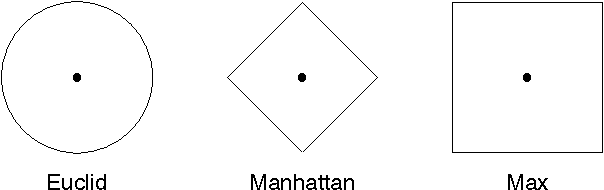
\includegraphics[scale=1]{fig7/distance.pdf}
\end{center}

\end{frame}

%---------------------------------------------------------------------

\begin{frame}%7
\frametitle{Beispiele für Distanzfunktionen /3}

\begin{itemize}
\item Für Datensätze $x= (x_1, \dots, x_d)$ mit kategorischen
  Attributswerten $x_i$:  
"`Anzahl der verschiedenen Werte"'
$$\dist_k(x,y)=\sum_{i=1}^d \delta(x_i,
y_i)\;\text{wobei}\;\delta(x_i,y_i) = 
\begin{cases}
0 & \text{wenn}\; x_i=y_i \\
1 & \text{wenn}\; x_i\neq y_i 
\end{cases}$$
\item Für endliche Mengen $x= \{x_1, \dots, x_d\}$: "`Anteil der
  verschiedenen Elemente in $x$ und $y$"'  
$$\dist_m(x, y) = \frac{|x \cup y| - |x \cap y|}{|x \cup y|}$$
\end{itemize}
\end{frame}

%---------------------------------------------------------------------

\begin{frame}%8
\frametitle{Beispiele für Distanzfunktionen /4}

\begin{itemize}
\item Für binäre Variable 
\begin{itemize}
\item Tabelle mit Werten für Ähnlichkeit 

\begin{center}
\begin{tabular}{|c||c|c|c|}
\hline
  & $1$ & $0$ & $\sum$ \\
\hline
\hline
$1$ & $a$ & $b$ & $a+b$ \\
\hline
$0$ & $c$ & $d$ & $c+d$ \\
\hline
$\sum$ & $a+c$ & $b+d$ & \\
\hline
\end{tabular}
\end{center}

\item Einfacher Ähnlichkeitskoeffizient 
$$d_S(x,y) = \frac{a+d}{a+b+c+d}$$
\item Jaccard Koeffizient 
$$d_J(x,y) = \frac{a}{c+b+d}$$
\end{itemize}
\end{itemize}

\end{frame}

%---------------------------------------------------------------------

\begin{frame}%8
\frametitle{Beispiele für Distanzfunktionen /5}

\begin{itemize}
\item Beispiel für binäre Variable 
{\footnotesize
\begin{tabular}{|c|c|c|c|c|c|c|c|}
\hline
Name & Geschlecht & Fieber & Husten & Test1 & Test2 & Test3 & Test4 \\
\hline
Jack & M & Y & N & P & N & N & N \\
Mary & F & Y & N & P & N & P & N \\
Jim  & M & Y & Y & N & N & N & N \\
\hline
\end{tabular}}

\begin{itemize}
\item $1 = (Y,P)$; $0 = (N)$
\begin{itemize}
\item $d_S$(Jack, Mary) $= \frac{5}{7} = 0.71$
\item $d_S$(Jack, Jim) $= \frac{4}{7} = 0.57$ 
\item $d_S$(Jim, Mary) $= \frac{3}{7} = 0.43$
\end{itemize}
\end{itemize}
\end{itemize}


\end{frame}

\begin{frame}%9
\frametitle{Partitionierende Verfahren}

\begin{itemize}
\item \hl{Prinzipielle Idee}
\begin{itemize}
\item Partitionierende Verfahren zerlegen eine Datenmenge in $k$
  Cluster, wobei gilt:  
\begin{itemize}
\item jeder Cluster enthält mindestens ein Objekt 
\item jedes Objekt gehört genau zu einem Cluster 
\end{itemize}
\end{itemize}
\item \hl{Konstruktion zentraler Punkte} [Forgy 1965] 
\begin{itemize}
\item Voraussetzung 
\begin{itemize}
\item Objekte sind Punkte $p=(x^p_1, \dots, x^p_d)$ in einem
  $d$-dimensionalen euklidischen Vektorraum; Verwendung der
  euklidischen Distanz für die Ähnlichkeit  
\end{itemize}
\item Zentroide 
\begin{itemize}
\item Jeder Cluster $C$ wird durch seinen Zentroid $\overline{x}_C$
  repräsentiert: $\overline{x}_C=(\overline{x}_1(C),
  \overline{x}_2(C), \dots, \overline{x}_d(C))$ 
\item $\overline{x}_j(C)=\frac{1}{n_C}\cdot\sum_{p\in C}x^p_j$ ist
  Mittelwert für die $j$-te Dimension der Punkte im Cluster $C$  
\item Zentroid eines Clusters ist anschaulich der Mittelwert aller
  Punkte des Clusters  
\end{itemize}
\end{itemize}
\end{itemize}

\end{frame}

%---------------------------------------------------------------------

\begin{frame}
\frametitle{Zentroide und Kompaktheit}

\begin{itemize}
\item \hl{Maß für die Kompaktheit eines Clusters}
\begin{itemize}
\item Summe der quadrierten euklidischen Distanzen zum Zentroid: 
$$TD^2(C) = \sum_{p \in C} \dist(p, \overline{x}_C)^2$$
\end{itemize}
\item \hl{Maß für die Kompaktheit eines Clustering}
\begin{itemize}
\item Summe der quadrierten Distanzen jedes Punktes zum Zentroid seines
Clusters: 
$$TD^2=\sum_{i=1}^k TD^2(C_i)$$
\end{itemize}

\end{itemize}

\end{frame}

%---------------------------------------------------------------------

\begin{frame}
\frametitle{Zentroide und Kompaktheit /2}

\begin{itemize}
\item \hl{Ziel}
\begin{itemize}
\item Zerlegung der Punktmenge in $k$ Klassen, so dass $TD^2$ minimal ist 
\item Interpretation: die $k$ Klassen werden so gebildet, dass die
  Varianz bezüglich der gegebenen Mittelwerte minimal wird ("`Varianz
  minimierende Techniken"')  
\item Umformulierung des Ausdrucks für $TD^2(C)$ zeigt Minimierung der
 Varianz: 
$$TD^2(C) = \sum_{p \in C}\sum_{j=1}^d (x^p_j - \overline{x}_j(C))^2$$
\end{itemize}
\end{itemize}

\end{frame}

%---------------------------------------------------------------------

\begin{frame}
\frametitle{Konstruktion von Zentroiden}

\begin{itemize}
\item \hl{Beispiel für k=3:}
\end{itemize} 


\begin{center}
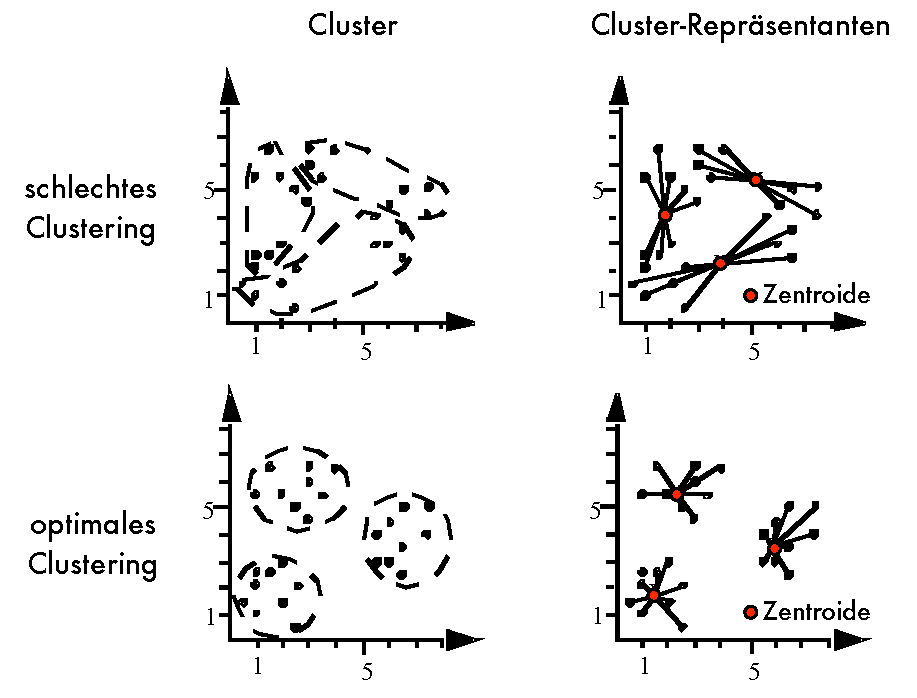
\includegraphics[scale=.5]{fig7/zentroiden-bsp.pdf}
\end{center}

\end{frame}

%---------------------------------------------------------------------

\begin{frame}
\frametitle{Algorithmus: Cluster durch  Varianzminimierung}

\begin{algo}
\textbf{ClusteringDurchVarianzMinimierung}(Punktmenge, $k$) \\
\1 \textrm{Erzeuge zufällig eine initiale Zerlegung der Punktmenge} \\
\2 \textrm{in $k$ Klassen;} \\
\1 \textrm{Berechne die Menge} $C'=\{C_1, \dots, C_k\}$ \textrm{der Zentroide} \\
\2 \textrm{für die $k$ Klassen;}  \\
\1 $C = \{\}$; \\
\1 \op{repeat until} $C = C'$ \\
\2 $C = C'$; \\
\2 \textrm{Bilde $k$ Klassen, durch Zuordnung jedes Punkts zum} \\
\3 \textrm{nächstliegenden Zentroid;}   \\ 
\2 \textrm{Berechne die Menge} $C'= \{C'_1, \dots, C'_k\}$ \textrm{der Zentroide} \\
\3 \textrm{für die neu bestimmten Klassen;} \\
\1 \op{return} $C$; \\
\end{algo}
\end{frame}
%---------------------------------------------------------------------

\begin{frame}
\frametitle{Cluster durch  Varianzminimierung: Beispiel}

\begin{center}
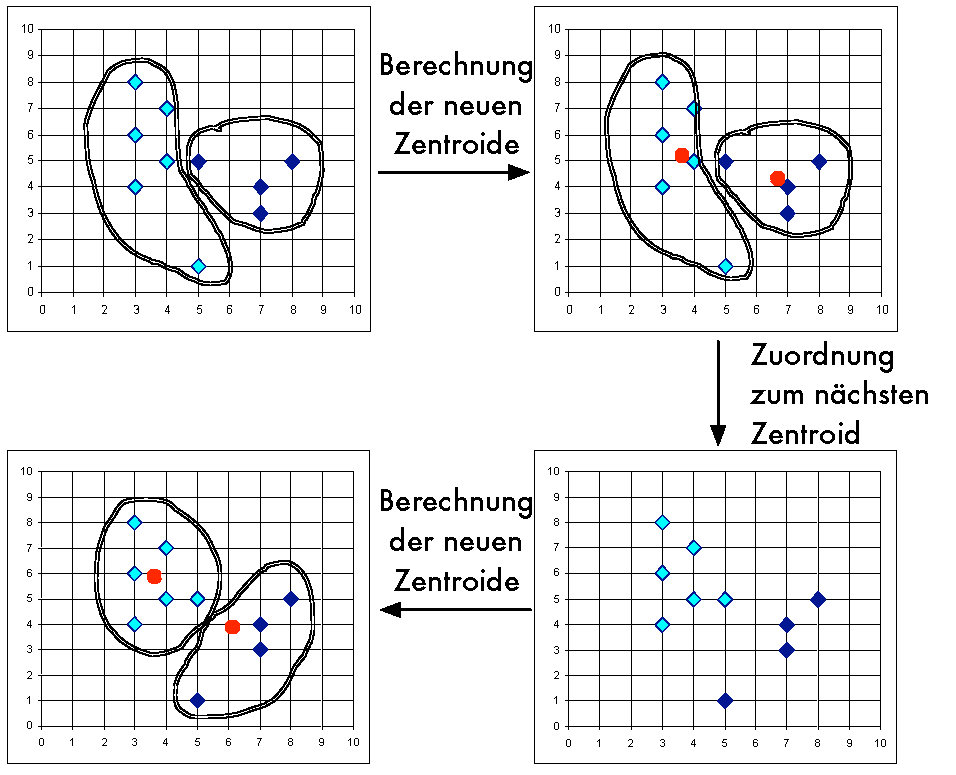
\includegraphics[scale=.5]{fig7/zentroiden-varianz.pdf}
\end{center}


\end{frame}

%---------------------------------------------------------------------

\begin{frame}
\frametitle{Cluster durch  Varianzminimierung /3}

\begin{itemize}
\item \hl{Eigenschaften des Algorithmus}
\begin{itemize}
\item Konvergiert gegen ein (möglicherweise nur lokales) Minimum 
\item Aufwand: $O(k \cdot n)$ für eine Iteration 
\item Anzahl der Iterationen ist im Allgemeinen klein ($\approx 5 -
  10$) 
\end{itemize}
\item \hl{weitere schwer quantifizierbare Eigenschaften}
\begin{itemize}
\item Anfälligkeit gegenüber Rauschen/Ausreißern 
\item konvexe Form der Cluster 
\item Ergebnis und Laufzeit hängen stark von der Initialisierung (der
  ersten zufälligen Zerlegung) ab  
\end{itemize}
\end{itemize}

\end{frame}

%---------------------------------------------------------------------

\begin{frame}
\frametitle{K-Means}

\begin{itemize}
\item \hl{Variante des Basisalgorithmus}
\begin{itemize}
\item Zentroide werden jedesmal direkt aktualisiert, wenn ein Punkt seine 
Clusterzugehörigkeit ändert 
\item Inkrementelle Anpassung, wenn ein Punkt $p$ vom Cluster $C_1$
  zum Cluster $C_2$ wechselt  
\begin{eqnarray*}
\overline{x}_j(C'_1) &=& \frac{1}{n_{C_1}-1}\cdot (n_{C_1} \cdot
\overline{x}_j(C_1)-x^p_j) \\
\overline{x}_j(C'_2) &=& \frac{1}{n_{C_2}+1}\cdot 
(n_{C_2} \cdot \overline{x}_j(C_2)+x^p_j) 
\end{eqnarray*}
$n_C$ gleich der Anzahl der Objekte in $C$
\end{itemize} 
\end{itemize}

\end{frame}

%---------------------------------------------------------------------

\begin{frame}
\frametitle{K-Means /2}

\begin{itemize}
\item \hl{Bemerkungen}
\begin{itemize}
\item bekannteste und am häufigsten angewendete partitionierende
  Clustering-Methode  
\item K-Means hat im Wesentlichen die gleichen Eigenschaften wie die
  obige Basismethode, ist aber zusätzlich noch stark
  reihenfolgeabhängig 
\end{itemize}
\item\hl{Variante ISODATA (Iterative Self-Organizing Data Analysis Techniques)}
\begin{itemize}
\item Verbesserung der Methode durch zusätzliche Operationen 
\begin{itemize}
\item Eliminiation sehr kleiner Cluster 
\item Verschmelzung von ähnlichen Clustern
\item Aufspalten von Cluster mit einer großen Standardabweichung
\end{itemize}
\item Problematisch: Parametrierung! 
\end{itemize}
\end{itemize}

\end{frame}


%---------------------------------------------------------------------
\begin{frame}[fragile]
\frametitle{K-Means in Python}

\begin{itemize}
\item Beispieldaten über Datengenerator: \texttt{make\_blobs} erzeugt Gauß-verteilte Daten für Clustering
\end{itemize}
\begin{minted}{python}
from sklearn.cluster import KMeans
from sklearn.datasets
  import make_blobs
  import matplotlib.pyplot as plt

data, l_true = make_blobs(n_samples=150, centers=3,
  cluster_std=0.5, random_state=0)
plt.scatter(data[:,0], data[:,1], s=50)
\end{minted}


\end{frame}
%---------------------------------------------------------------------

\begin{frame}[fragile]
\frametitle{K-Means in Python /2}

\begin{minted}{python}
labels = KMeans(n_clusters=3,
  random_state=0).fit_predict(data)
plt.scatter(data[:,0], data[:,1], c=labels, s=50)
\end{minted}

\begin{center}
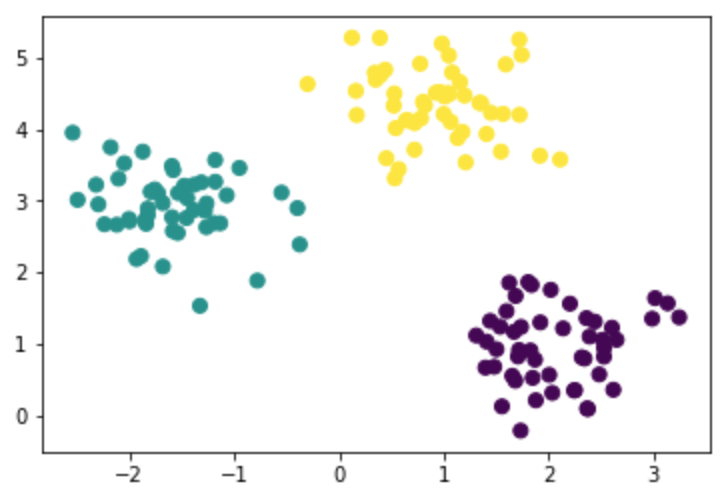
\includegraphics[scale=.5]{fig7/kmeans-blob.png}
\end{center}

\end{frame}

%---------------------------------------------------------------------

\begin{frame}[fragile]
\frametitle{K-Means in Python /3}

\begin{itemize}
\item Beispieldaten: Iris-Datensatz = 150 Objekte einer Schwertlilie (Iris)
\end{itemize}
\begin{minted}{python}
import seaborn as sb
iris = sb.load_dataset('iris')
data = iris.drop('species', axis=1)
labels = KMeans(n_clusters=3, random_state=0) 
         .fit_predict(data)
plt.scatter(data['sepal_length'], data['sepal_width'], 
  c=labels, s=50)
\end{minted}
\end{frame}

\begin{frame}[fragile]
\frametitle{K-Means in Python /3}

Was passiert bei nicht-konvexen Clustern?
\begin{minted}{python}
from sklearn.datasets import make_moons
data, l = make_moons(150, noise=0.05, random_state=0)
labels = KMeans(n_clusters=2, random_state=0).fit_predict(data)
\end{minted}

\vspace*{-.5cm}
\begin{center}
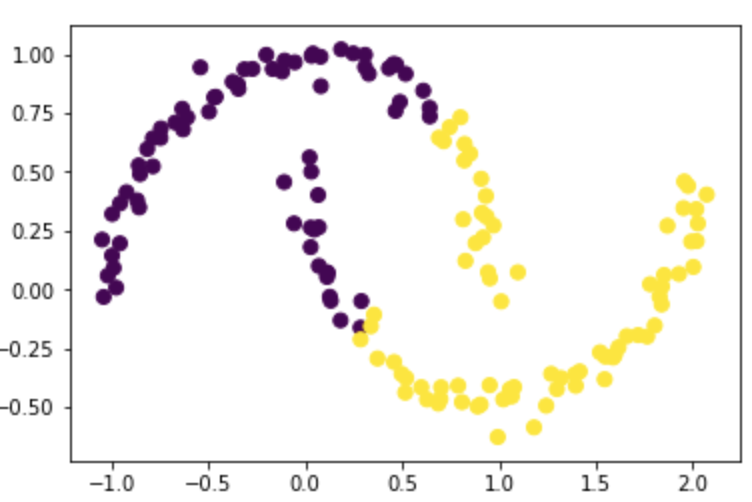
\includegraphics[scale=.5]{fig7/kmeans-moon.png}
\end{center}

\end{frame}

%---------------------------------------------------------------------

\begin{frame}
\frametitle{Auswahl repräsentativer Punkte}

\begin{itemize}
\item\hl{Voraussetzung}
\begin{itemize}
\item Beliebige Objekte und eine beliebige Distanzfunktion zur
  Modellierung der Ähnlichkeit 
\end{itemize}
\item\hl{Medoide} 
\begin{itemize}
\item Repräsentation eines Clusters $C$ (repräsentativer Punkt /
 "`zentralstes"' Objekt)  
\item Unterschied zu einem Zentroid: Medoid ist ein Objekt, welches
  auch in der Datenmenge vorkommt 
\end{itemize}
\end{itemize}
\end{frame}

%---------------------------------------------------------------------

\begin{frame}

\frametitle{Auswahl repräsentativer Punkte /2}

\begin{itemize}
\item\hl{Maß für die Kompaktheit eines Clusters}
\begin{itemize}
\item Summe der Distanzen zum Medoid 
$$TD(C) = \sum_{p \in C} \dist(p, m_C)$$
\end{itemize}
\item\hl{Maß für die Kompaktheit eines Clustering} 
\begin{itemize}
\item Summe der Distanzen jedes Punktes zum Medoid seines Clusters 
$$TD=\sum_{i=1}^k TD(C_i)$$
\end{itemize}
\item\hl{Ziel: Bestimmung von $k$ Medoiden, so dass $TD$ minimal ist} 
\end{itemize}
\end{frame}

%---------------------------------------------------------------------

\begin{frame}
\frametitle{Konstruktion von Medoiden}

\begin{itemize}
\item\hl{Beispiel für k=3:} 

\begin{center}
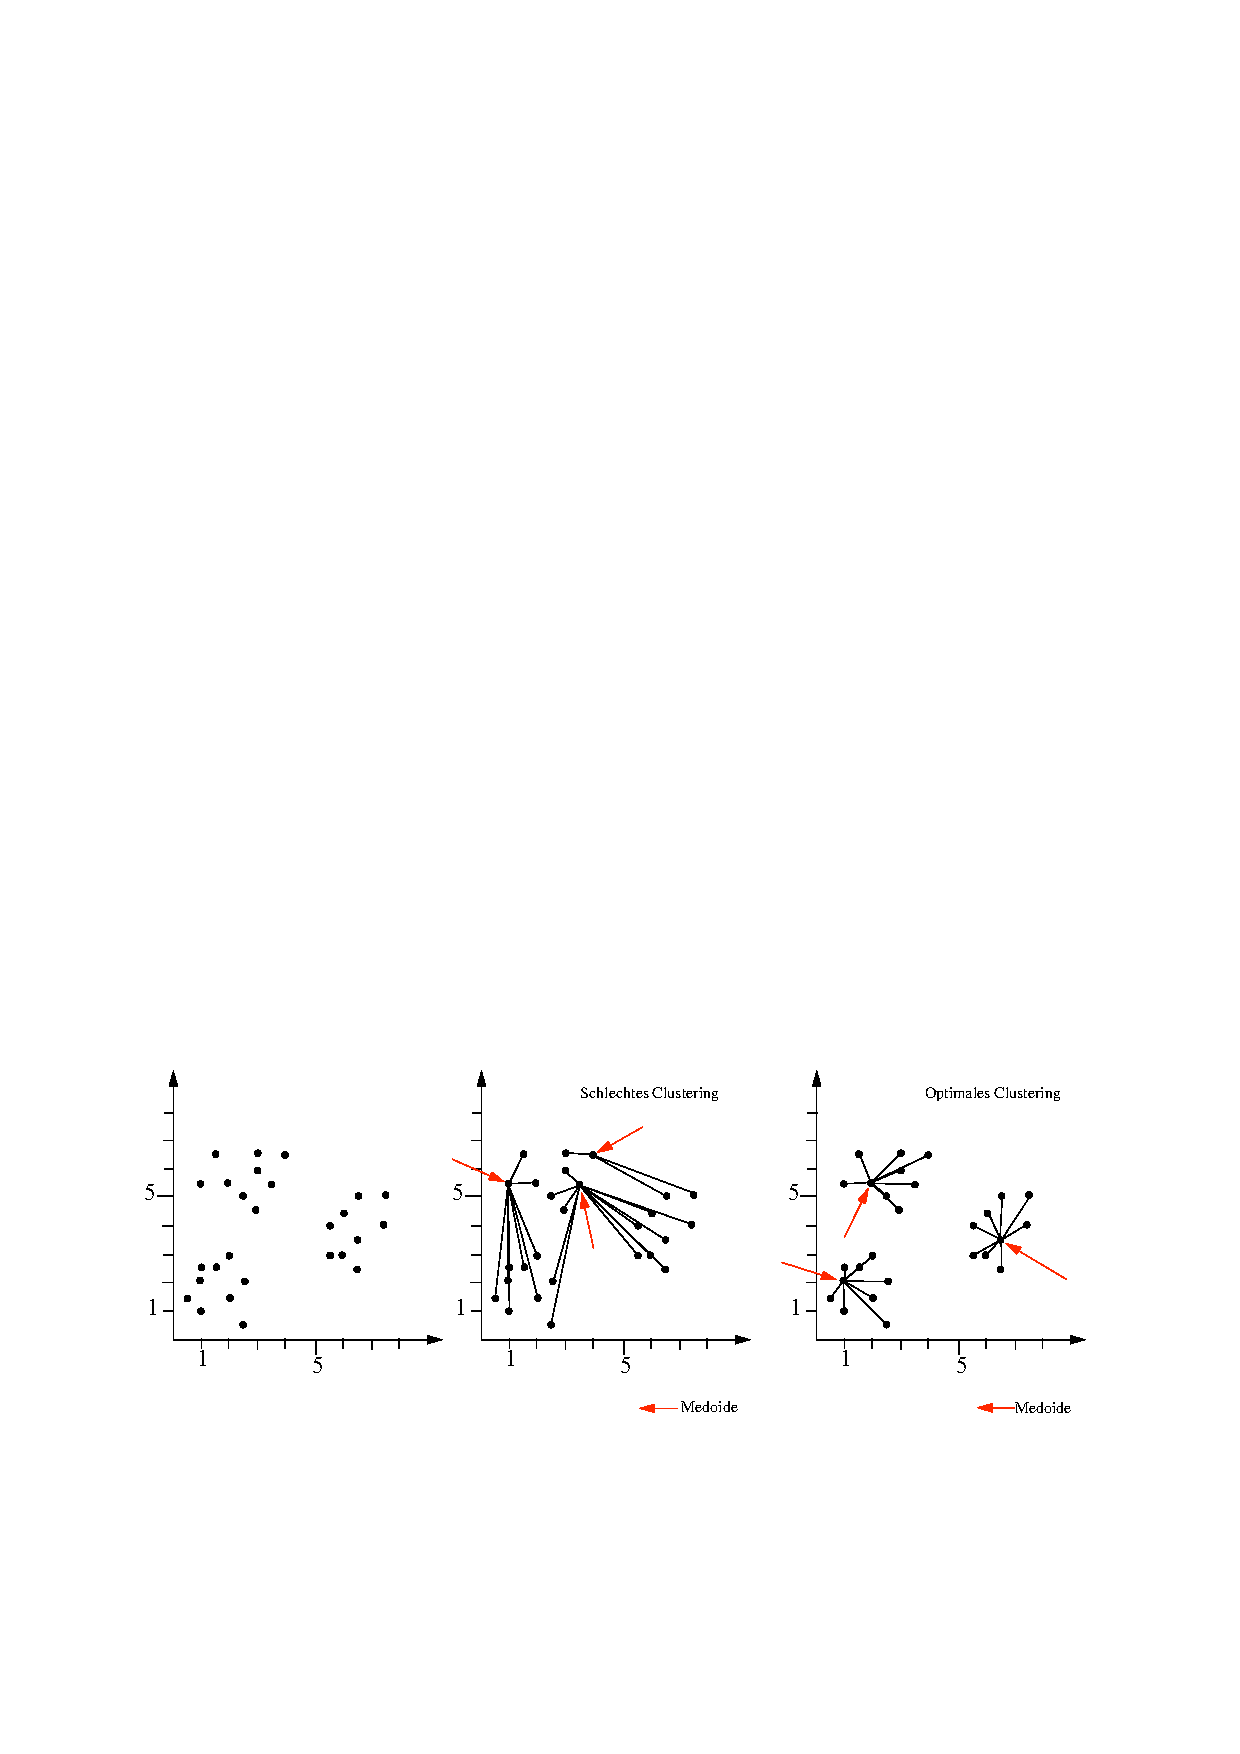
\includegraphics[scale=.6]{fig7/medoide.pdf}
\end{center}

\item\hl{Idee zum PAM-Algorithmus}
\begin{itemize}
\item Vertausche in jedem Schritt ein Medoid mit einem Nicht-Medoid 
\item Auswahl des Paares, welches die größte Reduktion der Kosten von
  $TD$ bewirkt  
\end{itemize}
\end{itemize}

\end{frame}

%---------------------------------------------------------------------

\begin{frame}
\frametitle{Partitioning Around Medoids (PAM)}

\begin{algo}
\textbf{PAM}(Objektmenge, $k$, dist) \\
\1 \textrm{Initialisiere die $k$ Medoidkandidaten} \\
\1 TD\_Änderung := $-\infty$; \\
\1 \op{while} TD\_Änderung $< 0$ \op{do} \\
\2 \textrm{Berechne für jedes Paar (Medoid $M$, Nicht-Medoid $N$)}\\
\3 \textrm{den Wert} TD$_{N\leftrightarrow M}$, \textrm{d.h. den Wert} TD \\
\3 \textrm{unter der Annahme, dass der Medoid $M$} \\
\3 \textrm{durch den Nicht-Medoid $N$ ersetzt wird;}  \\
\2 \textrm{Wähle das Paar $(M, N)$ für das} \\
\3 TD\_Änderung := TD$_{N\leftrightarrow M}$ - TD \textrm{minimal ist;} \\
\2\op{if} TD\_Änderung $< 0$ \op{then} \\
\3 \textrm{ersetze den Medoid $M$ tatsächlich durch den Nicht-Medoid $N$;} \\
\3 \textrm{speichere die aktuellen Medoide als die} \\
\4 \textrm{bisher beste Partionierung} 
\end{algo}

\end{frame}

%---------------------------------------------------------------------

\begin{frame}
\frametitle{Algorithmus: PAM /2}

\begin{itemize}

\item\hl{Eigenschaften des Algorithmus}
\begin{itemize}
\item Greedy-Verfahren: Konvergiert gegen ein (möglicherweise nur
  lokales) Minimum  
\item Ergebnis und Laufzeit hängen nicht von der Reihenfolge, in der
  die Objekte gespeichert sind, ab (in Gegensatz zu K-Means). 
\item Größtes Problem des Algorithmus PAM ist seine enorme Laufzeit
  $\rightarrow$ kleine Datenmengen   
\end{itemize}
\end{itemize}

\end{frame}

\begin{frame}
\frametitle{PAM: Varianten}

\begin{itemize}
\item\hl{CLARA (Clustering Large Applications)}
\begin{itemize}
\item PAM auf mehrere Stichproben; Auswahl des besten Clustering-Ergebnisses 
\item größere Datenmenge, aber Entscheidung nur auf Stichproben! 
\end{itemize}
\item\hl{CLARANS -- Clustering Large Applications based on RANdomized Search}
\begin{itemize}
\item Betrachtung von höchstens \texttt{maxneighbor} viele zufällig ausgewählten
  Paaren  
\item Durchführung der ersten Ersetzung, die überhaupt eine
  Reduzierung des $TD$-Wertes bewirkt 
\item Suche nach $k$ "`optimalen"' Medoiden wird \texttt{numlocal} mal wiederholt 
\end{itemize}
\end{itemize}

\end{frame}

%---------------------------------------------------------------------


\begin{frame}
\frametitle{Bestimmung der natürlichen Anzahl von Clustern}

\begin{itemize}
\item \hl{bisher} 
\begin{itemize}
\item Wert $k$ für die Anzahl der Cluster vom Benutzer vorgegeben 
\item "`richtige"' Anzahl der Cluster unbekannt ist in vielen
  Anwendungen jedoch unbekannt  
\end{itemize}
\item \hl{Bestimmung der Anzahl von Clustern}
\begin{itemize}
\item $k$-fache Anwendung der K-Means- oder K-Medoid-Verfahren 
\item Auswahl des besten "`Cluster"'-Ergebnisses 
\item Güte eines Clusterings 
\begin{itemize}
\item Kompaktheit eines Clusterings, d.h. $TD^2$ bzw. $TD$ ungeeignet 
\item besser: Silhouetten-Koeffizient 
\end{itemize}
\end{itemize}
\end{itemize}

\end{frame}

%---------------------------------------------------------------------

\begin{frame}
\frametitle{Bestimmung der natürlichen Anzahl von Clustern /2}

\begin{itemize}
\item \hl{Verallgemeinerte Abstände}
\begin{itemize}
\item Durchschnittlicher Abstand des Objekts $o$ zu einem Cluster
  $C_i$:  
$$\dist(o,C_i)=\frac{\sum_{p\in C_i}\dist(o,p)}{|C_i|}$$
\item Durchschnittlicher Abstand des Objekts $o$ zu "`seinem"' Cluster
  $C$: $a(o) = \dist(o,C)$ 
\item Durchschnittlicher Abstand des Objekts $o$ zum "`Nachbar-Cluster"': 
$b(o)=\displaystyle\min_{C_i \in C_M, C_i\neq C} \dist(o, C_i)$
\end{itemize}
\end{itemize}

\end{frame}

%---------------------------------------------------------------------

\begin{frame}
\frametitle{Silhouetten}

\begin{itemize}
\item \hl{Silhouette eines Objekts}
$$
s(o)=
\begin{cases}
0 & \text{wenn}\;|C|=1,\;\text{d.h.}\;a(o)=0 \\
\frac{b(o)-a(o)}{\max\{a(o),b(o)\}}\;&\text{sonst}
\end{cases}
$$
 mit $-1 \leq s(o) \leq 1$ 
\begin{itemize}
\item Interpretation der Silhouette eines Objekts 
\begin{itemize}
\item $s(o) \approx 0$, d.h. $a(o)\approx b(o)$, $o$ liegt ungefähr
  zwischen seinem eigenen und dem Nachbarcluster  
\item $s(o) \approx 1$, d.h. $a(o)$ ist wesentlich kleiner als $b(o)$,\\
  $o$ ist gut klassifiziert  
\item $s(o) \approx -1$, d.h. $b(o)$ ist wesentlich kleiner als
  $a(o)$,\\ $o$ ist schlecht klassifiziert  
\end{itemize}
\end{itemize}
\end{itemize}
\end{frame}

%---------------------------------------------------------------------


\begin{frame}
\frametitle{Silhouetten /2}

\begin{itemize}
\item \hl{Silhouetten-Koeffizient eines Clustering $C_M$:}
$$s(C_M) = \frac{\displaystyle\sum_{C\in C_M} \displaystyle\sum_{o \in C} s(o)}{|O|}$$
\begin{itemize}
\item Maß für die Güte eines Clustering, welches unabhängig von der
  Anzahl $k$ der Cluster ist  
\item Je höher der Wert $s(C_M)$, desto besser ist das Clustering
\end{itemize}
\item\hl{Interpretation des Silhouetten-Koeffizienten}
\begin{itemize}
\item starke Struktur: $0.70 < s(C_M) \leq 1.00$ 
\item brauchbare Struktur: $0.50 < s(C_M) \leq 0.70$ 
\item schwache Struktur: $0.25 < s(C_M) \leq 0.50$ 
\end{itemize}
\end{itemize}
\end{frame}

%---------------------------------------------------------------------

\begin{frame}
\frametitle{Silhouetten /3}

\begin{center}
%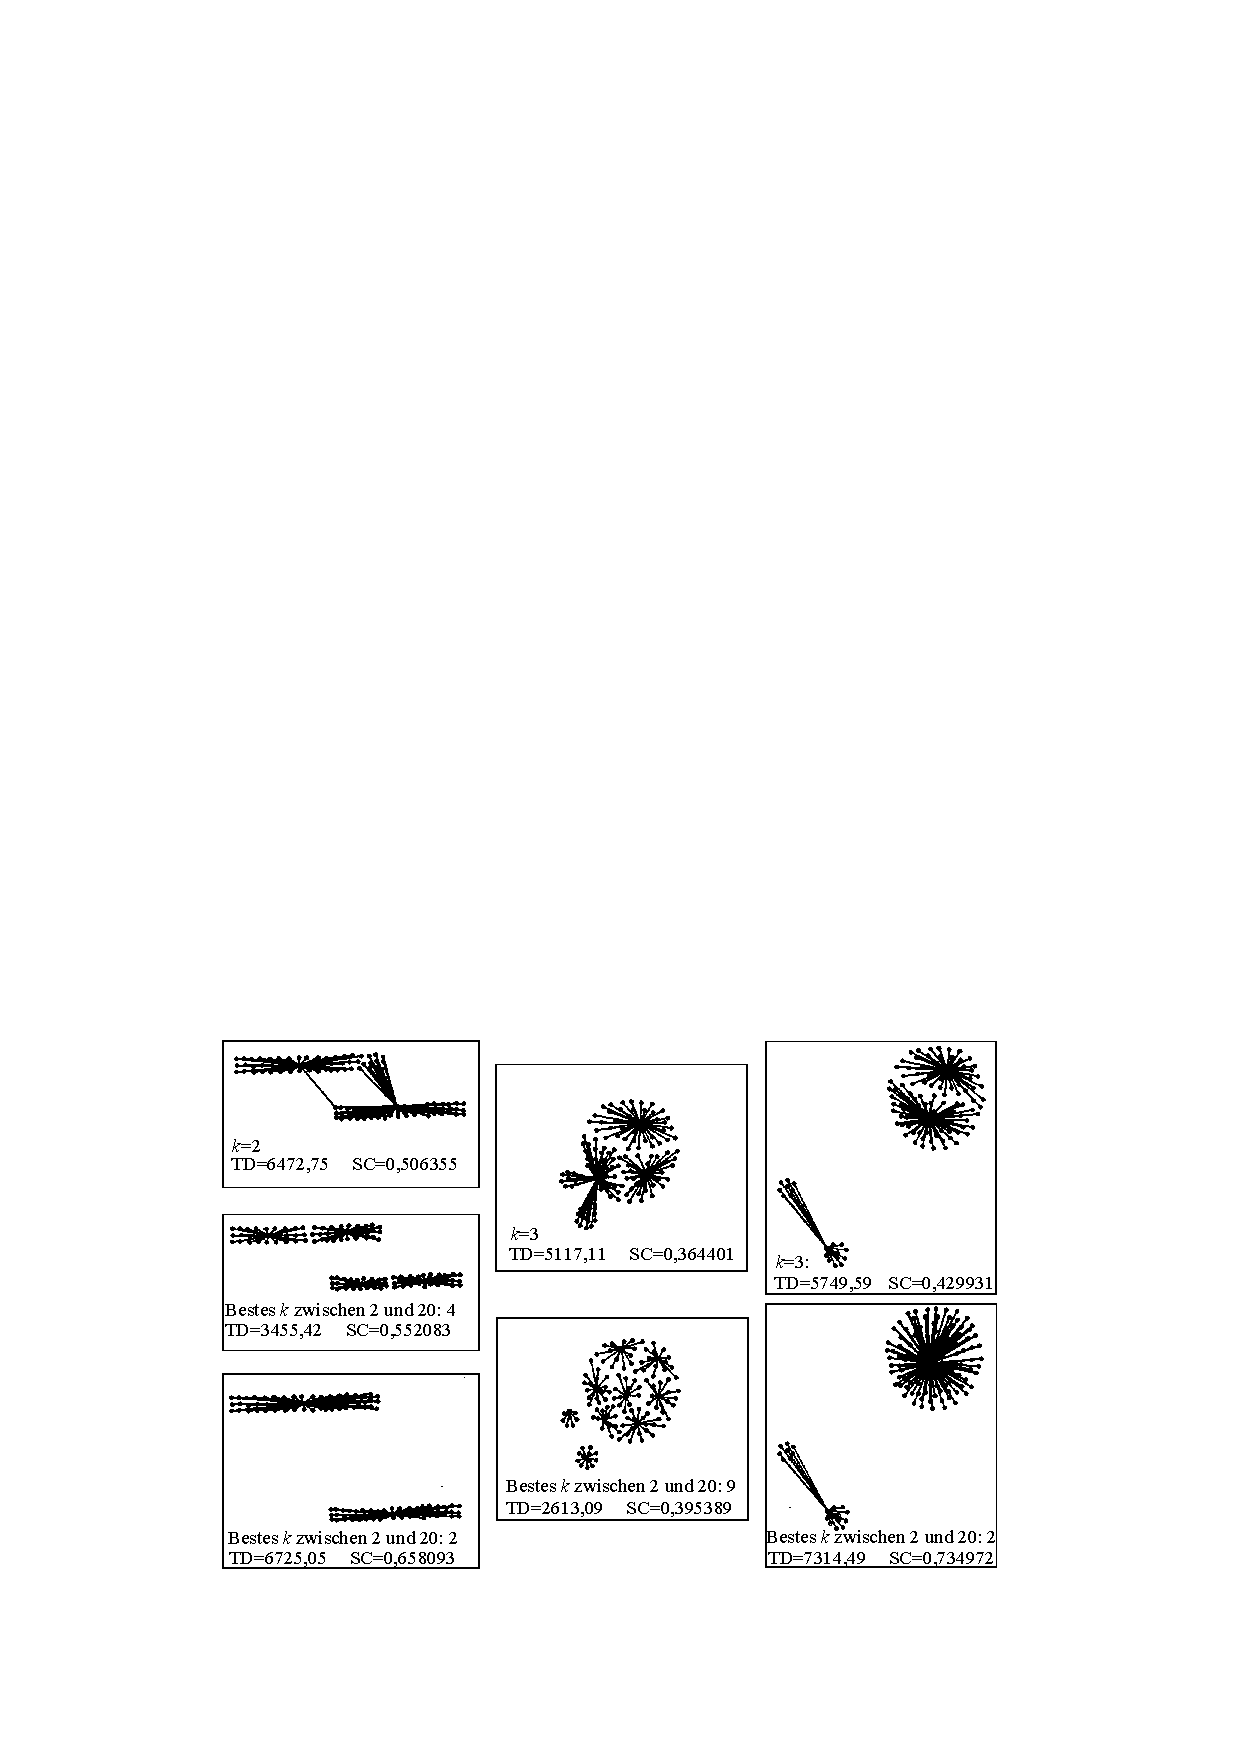
\includegraphics[scale=.7]{fig7/silhouetten.pdf}
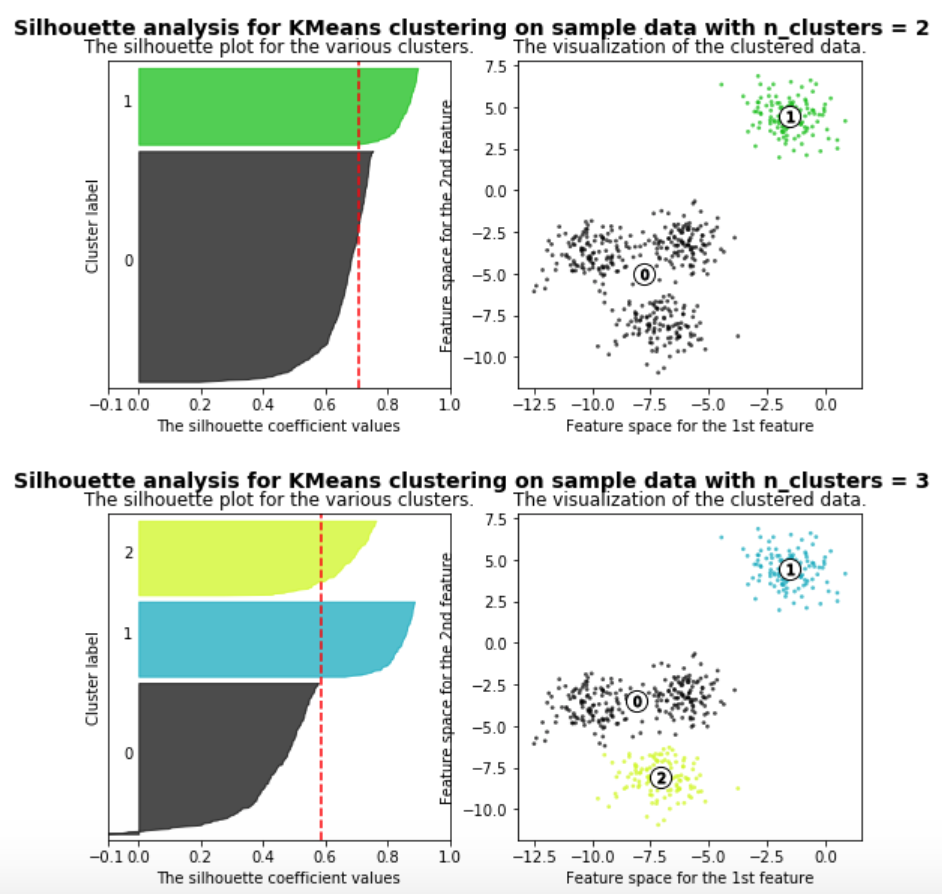
\includegraphics[scale=.32]{fig7/silhouetten-1.png}
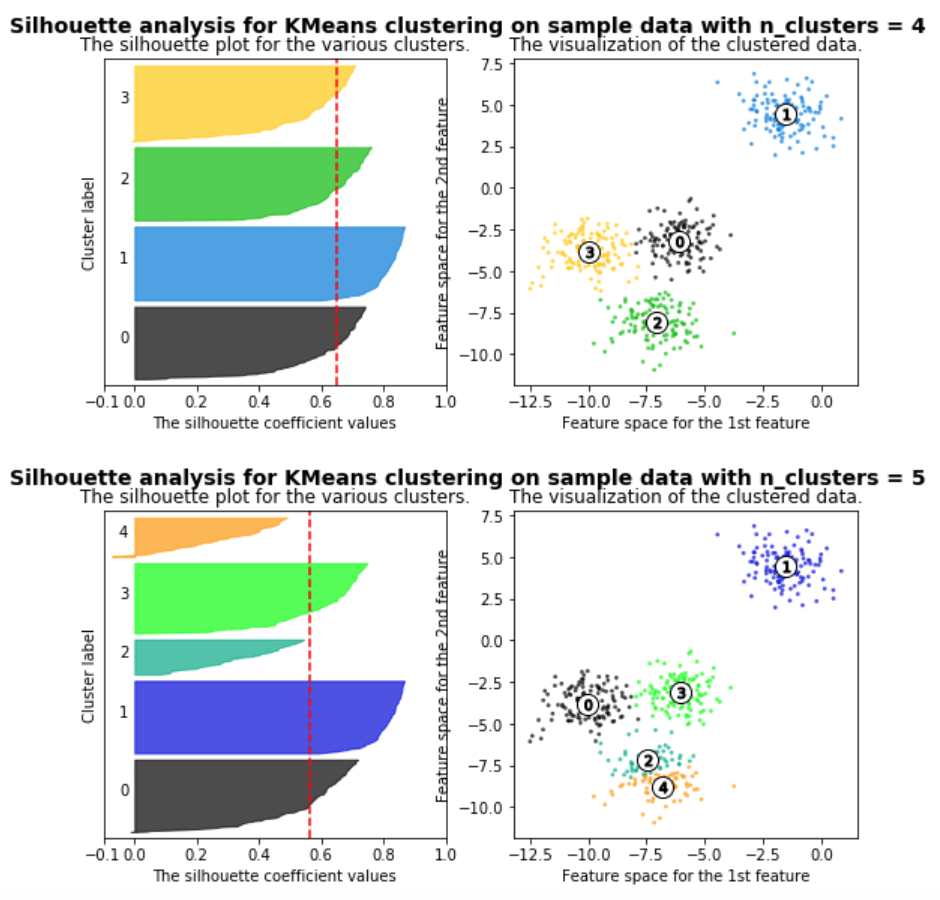
\includegraphics[scale=.32]{fig7/silhouetten-2.png}
\end{center}

\url{https://scikit-learn.org/stable/auto_examples/cluster/plot_kmeans_silhouette_analysis.html}

\end{frame}


\section{Klassifikation}


%---------------------------------------------------------------------

\frame{
  \frametitle{Überblick}
  \tableofcontents[currentsection,hidesubsections,firstsection=28]
}

\begin{frame}
\frametitle{Klassifikationsproblem}

\begin{itemize}
\item Gegeben: 
\begin{itemize}
\item Grundgesamtheit $G$ von zu klassifizierenden Objekten
\item eine Menge $O \subset G$ von Objekten des Formats $(o_1, \dots,
  o_d)$ mit Attributen $A_i$, $1 \leq i \leq d$, und
  Klassenzugehörigkeit $c_i$, $c_i \in C = \{c_1, \dots, c_k \}$
\end{itemize}
\item Gesucht:
\begin{itemize}
\item die Klassenzugehörigkeit für Objekte aus $D \setminus O$ 
\item ein Klassifikator $K: D \rightarrow C$
\end{itemize} 
\item Abgrenzung zum Clustering
\begin{itemize}
\item Klassifikation: Klassen apriori bekannt
\item Clustering: Klassen werden erst gesucht
\end{itemize}
\item Verwandtes Problem: Vorhersage (Prediction)
\begin{itemize}
\item gesucht ist der Wert für ein numerisches Attribut 
\item Methode z.B. Regression
\end{itemize}
\end{itemize}

\end{frame}

%---------------------------------------------------------------------

\begin{frame}
\frametitle{Beispiel}

\begin{center}
{\footnotesize\begin{tabular}{|c|c|c|c|c|}
\hline
Kunden-ID & Schulden & Einkommen & Ang.verhältnis & Risiko \\
\hline\hline
1 & Hoch & Hoch & Selbständig & Hoch \\
2 & Hoch & Hoch & Angestellt & Hoch \\
3 & Hoch & Niedrig & Angestellt & Hoch \\
4 & Niedrig & Niedrig & Angestellt & Niedrig \\
5 & Niedrig & Niedrig & Selbständig & Hoch \\
6 & Niedrig & Hoch & Angestellt & Niedrig \\
\hline
\end{tabular}}
\end{center}

\begin{itemize}
\item Einfacher Klassifikator
\end{itemize}
\begin{smallalgo}
\op{if} Schulden $=$ Hoch \op{then} Risiko $=$ Hoch;\\
\op{if} Schulden $=$ Niedrig \op{and} Ang.verhältnis $=$ Angestellt \\
\1 \op{then} Risiko $=$ Niedrig;\\
\op{if} Schulden $=$ Niedrig \op{and} Ang.verhältnis $=$ Selbständig \\
\1 \op{then} Risiko = Hoch
\end{smallalgo}

\end{frame}

%---------------------------------------------------------------------

\begin{frame}
\frametitle{Prozess: Konstruktion des Modells}

\begin{center}
{\tiny\begin{tabular}{|c|c|c|c|c|}
\hline
Kunden-ID & Schulden & Einkommen & Anstellungs- & Risiko \\
           &           &            & verhältnis   &  \\
\hline\hline
1 & Hoch & Hoch & Selbständig & Hoch \\
2 & Hoch & Hoch & Angestellt & Hoch \\
3 & Hoch & Niedrig & Angestellt & Hoch \\
4 & Niedrig & Niedrig & Angestellt & Niedrig \\
5 & Niedrig & Niedrig & Selbständig & Hoch \\
6 & Niedrig & Hoch & Angestellt & Niedrig \\
\hline
\end{tabular}}
\end{center}
\begin{center}
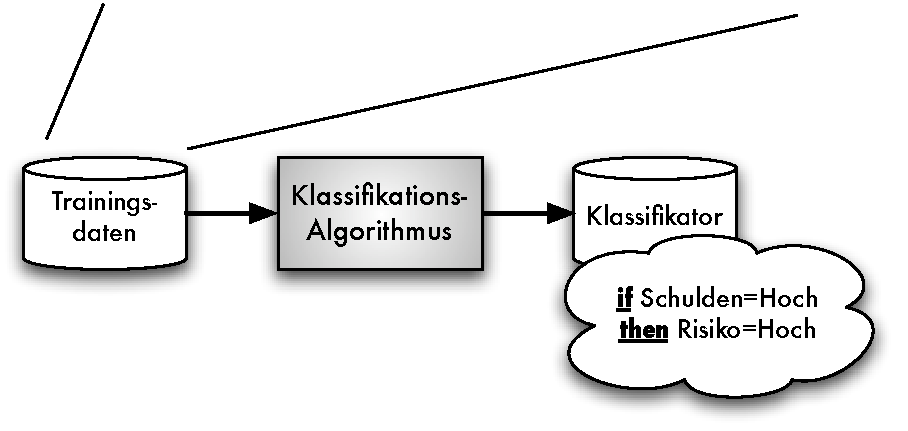
\includegraphics[scale=.6]{fig7/klass-prinzip-modell.pdf}
\end{center}


\end{frame}

%---------------------------------------------------------------------

\begin{frame}
\frametitle{Prozess: Anwendung des Modells}

\begin{center}
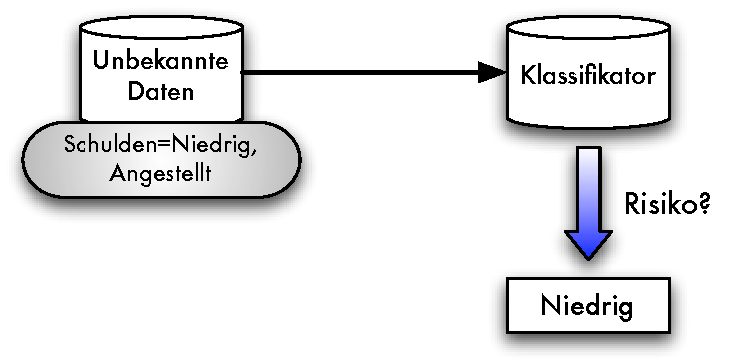
\includegraphics[scale=.7]{fig7/klass-prinzip-anw.pdf}
\end{center}

\begin{itemize}
\item manchmal:
\begin{itemize}
\item keine Klassifikation unbekannter Daten
\item sondern "`nur"' besseres Verständnis der Daten
\end{itemize}
\end{itemize}

\end{frame}

\begin{frame}
\frametitle{Entscheidungsbaumverfahren}

\begin{center}
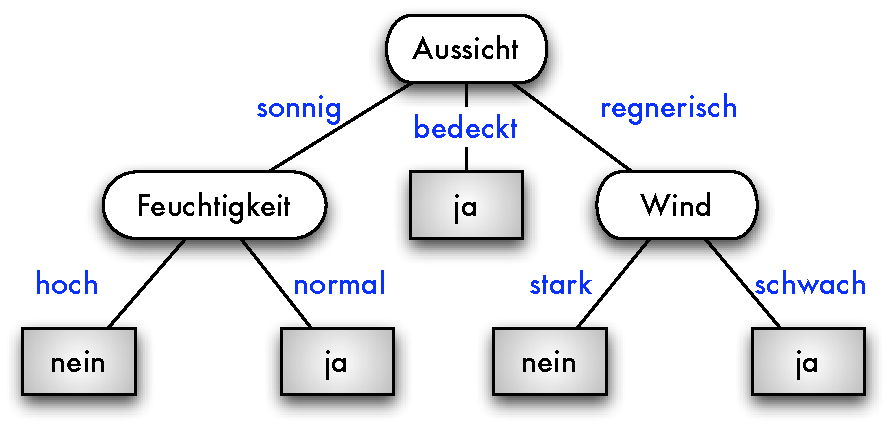
\includegraphics[scale=.7]{fig7/entscheidungsbaum-tennis.pdf}
\end{center}

\begin{itemize}
\item Finden von explizitem Wissen
\item Entscheidungsbäume für die meisten Nutzer verständlich
\end{itemize}

\end{frame}

%---------------------------------------------------------------------

\begin{frame}
\frametitle{Grundbegriffe}

\begin{itemize}
\item \hl{Entscheidungsbaum} ist ein Baum mit folgenden Eigenschaften:
\begin{itemize}
\item ein innerer Knoten repräsentiert ein Attribut,
\item eine Kante repräsentiert einen Test auf dem Attribut des Vaterknotens,
\item ein Blatt repräsentiert eine der Klassen
\end{itemize}
\item \hl{Konstruktion eines Entscheidungsbaums}
\begin{itemize}
\item anhand der Trainingsmenge 
\item Top-Down 
\end{itemize}
\item \hl{Anwendung eines Entscheidungsbaums}
\begin{itemize}
\item Durchlauf des Entscheidungsbaum von der Wurzel zu einem der
  Blätter $\leadsto$ eindeutiger Pfad  
 \item Zuordnung des Objekts zur Klasse des erreichten Blatts
\end{itemize}
\end{itemize}
\end{frame}

%---------------------------------------------------------------------

\begin{frame}
\frametitle{Konstruktion eines Entscheidungsbaums}

\begin{itemize}
\item Basis-Algorithmus
\end{itemize}

\begin{smallalgo}
\textbf{ConstructTree}(Trainingsmenge $T$, \op{float} min-conf)\\
\1 \op{if} \textrm{mind.} min-conf \textrm{der Objekte aus} $T$ \textrm{in Klasse} $c$ \op{then} \\
\2 \op{return}; \\
\1 \op{else} \\
\2 \op{for each} \textrm{Attribut} $A$ \op{do} \\
\3 \op{for each} \textrm{möglicher Split von} $A$ \op{do} \\
\4 \textrm{bewerte Qualität der Partitionierung, die durch Split entstehen
würde}; \\
\2 \textrm{führe besten aller dieser Splits durch}; \\
\2 $T_1, T_2, \dots, T_m$ := \textrm{durch diesen Split entstehende
Partitionen von} $T$; \\
\2 ConstructTree($T_1$, min-conf); \\
\2 \dots \\
\2 ConstructTree($T_m$, min-conf);
\end{smallalgo}

$\leadsto$ lokal optimierender Algorithmus (Greedy-Verfahren)

\end{frame}

%---------------------------------------------------------------------

\begin{frame}[shrink]
\frametitle{Beispiel}

%\vspace*{-2em}
\begin{center}
{\footnotesize\begin{tabular}{|c|l|l|l|l|l|}
\hline
Tag & Aussicht & Temperatur & Feuchtigkeit & Wind & Tennisspielen \\
\hline\hline
1 & sonnig & heiß & hoch & schwach & nein \\ \hline
2 & sonnig & heiß & hoch & stark & nein \\ \hline
3 & bedeckt & heiß & hoch & schwach & ja \\ \hline
4 & regnerisch & mild & hoch & schwach & ja \\ \hline
5 & regnerisch & kühl & normal & schwach & ja \\ \hline
6 & regnerisch &  kühl & normal & stark & nein \\ \hline
7 & bedeckt & kühl & normal & stark & ja \\ \hline
8 & sonnig &  mild & hoch & schwach & nein \\ \hline
9 & sonnig & kühl & normal & schwach & ja \\ \hline
10 & regnerisch & mild & normal & schwach & ja \\ \hline
11 & sonnig & mild & normal & stark & ja \\ \hline
12 & bedeckt & mild & hoch & stark & ja \\ \hline
13 & bedeckt & heiß & normal & schwach & ja \\ \hline
14 & regnerisch & mild & hoch & stark & nein \\ \hline
\end{tabular}}

\vspace*{1em}
\hl{Ist heute ein guter Tag zum Tennis spielen?}
\end{center}

\end{frame}

%---------------------------------------------------------------------

\begin{frame}
\frametitle{Beispiel /2}

\begin{center}
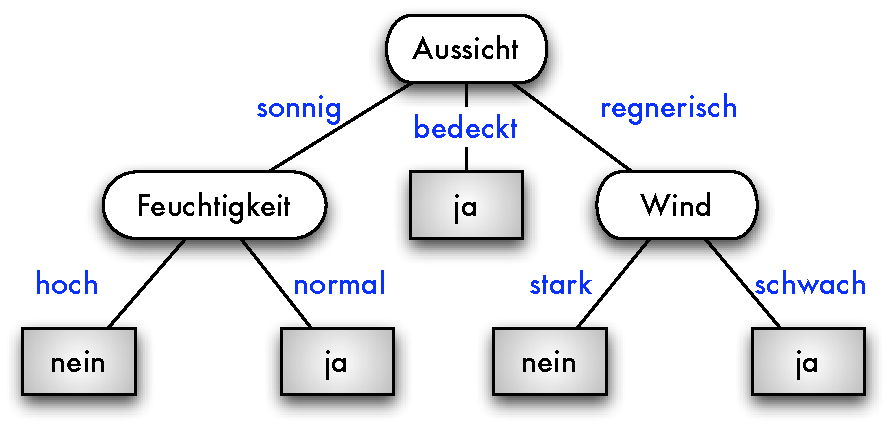
\includegraphics[scale=.7]{fig7/entscheidungsbaum-tennis.pdf}
\end{center}

\end{frame}

%---------------------------------------------------------------------
\begin{frame}
\frametitle{Entscheidungsbaumkonstruktion}

\begin{itemize}
\item \hl{Prinzip}: 
\begin{itemize}
\item Partitionierung der Datensätze basierend auf einem Attributest
  (Split-Bedingung), der nach einem bestimmtes Kriterium optimiert
\end{itemize}

\item \hl{Fragestellungen}:
\begin{itemize}
\item Spezifikation der Split-Bedingung
\item bester Split
\item Abbruchbedingung
\end{itemize}
\end{itemize}
\end{frame}

%---------------------------------------------------------------------
\begin{frame}
\frametitle{Split-Bedingung}

\begin{itemize}
\item Split-Strategie ist Kern des Entscheidungsbaum-Klassifikators
\item abhängig vom Typ des Attributs
\begin{itemize}
\item kategorisch (z.B. heiß, mild, kühl)
\item numerisch (z.B. Temperatur in $^\circ$C)
\end{itemize}
\item Anzahl der Partitionen nach Split
\begin{itemize}
\item binärer Split (z.B. Wind = "`stark/schwach"')
\item Mehrwege-Split (für jede Ausprägung)
\end{itemize}
\end{itemize}

\end{frame}

%---------------------------------------------------------------------
\begin{frame}
\frametitle{Split für kategorische Attribute}

\begin{itemize}
\item Mehrwege-Split: soviele Partitionen wie Ausprägungen im
  Wertebereich des Attributs 
\begin{center}
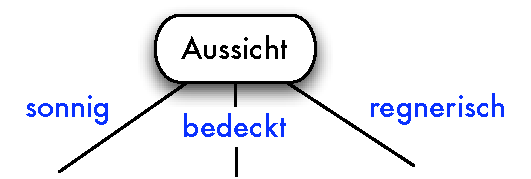
\includegraphics[scale=.5]{fig7/split-kat1.pdf}
\end{center}
\item Binärer Split:
\begin{itemize}
\item Test der Form \emph{Attribut} $= a$ : genau ein Split
\item Test der Form \emph{Attribut} $\in M$ : $O(2^m)$ verschiedene
  Splits bei $m=|M|$  
\begin{itemize}
\item Aufteilung der Werte in zwei disjunkte Teilmengen
\item optimale Partitionierung?
\end{itemize}
\end{itemize}
\begin{center}
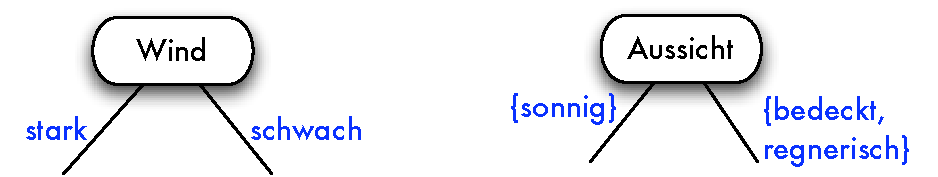
\includegraphics[scale=.5]{fig7/split-kat2.pdf}
\end{center}
\end{itemize}

\end{frame}

%---------------------------------------------------------------------

\begin{frame}
\frametitle{Split für numerische Attribute}

\begin{itemize}
\item Diskretisierung: Abbildung auf kategorische Werte
  (z.B. Temperatur in $^\circ$C $\Longrightarrow$ \{ kühl, mild, heiß
  \})
\begin{itemize}
\item statisch: vor Konstruktion des Entscheidungsbaums
\item dynamisch: Konstruktion geeigneter Intervalle (gleichgroße
  Bereiche, Häufigkeiten, durch Clustering)
\end{itemize}
\item Binäre Entscheidung: \emph{Attribut}$< a$
  bzw. \emph{Attribut}$\geq a$
\begin{itemize}
\item Analyse aller möglichen Partitionierungen (Werte von $a$)
\item berechnungsintensiv
\end{itemize}

\begin{center}
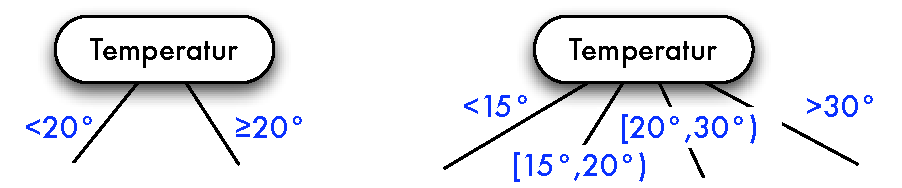
\includegraphics[scale=.5]{fig7/split-num.pdf}
\end{center}
\end{itemize}

\end{frame}

%---------------------------------------------------------------------

\begin{frame}
\frametitle{Bester Split}

\begin{itemize}
\item vor Partitionierung: 14 Datensätze (ja: 9, nein: 5)
\end{itemize}

\begin{center}
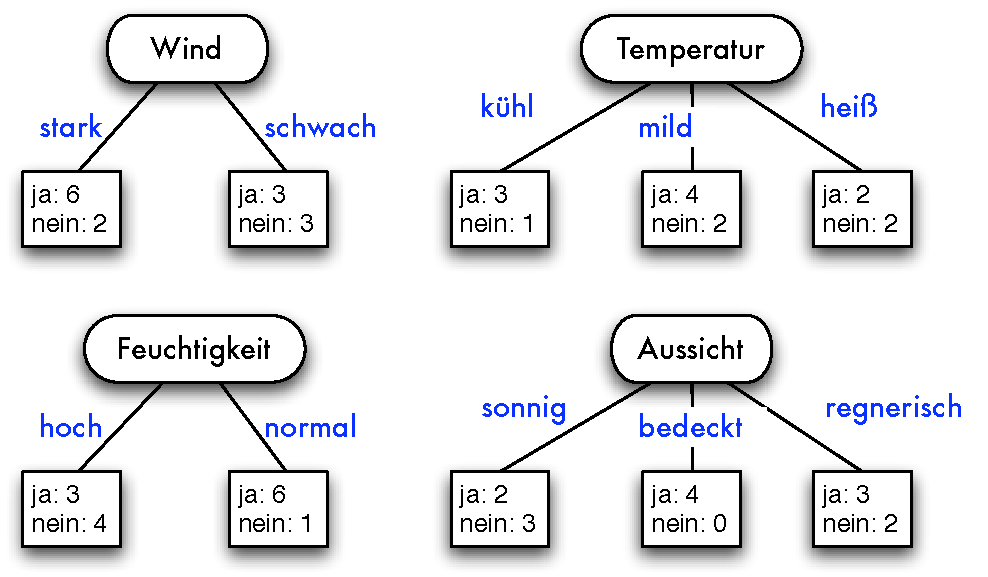
\includegraphics[scale=.5]{fig7/split-bewertung.pdf}
\end{center}

\begin{center}
\only<2->{\alert{Welche Split-Bedingung soll gewählt werden?}}
\end{center}
\end{frame}

%---------------------------------------------------------------------
\begin{frame}
\frametitle{Qualitätsmaße für Splits}

\begin{itemize}
\item Gegeben:
\begin{itemize}
\item eine Menge $T$ von Trainingsobjekten
\item eine disjunkte, vollständige Partitionierung $T_1, T_2, \dots,
  T_m$  von $T$ 
\item $p_i$ die relative Häufigkeit der Klasse $c_i$ in $T$
\end{itemize}
\item Gesucht:
\begin{itemize}
\item ein Maß der \hl{Unreinheit} einer Menge $S$ von
  Trainingsobjekten in Bezug  auf  die Klassenzugehörigkeit  
\item ein Split von $T$ in $T_1, T_2, \dots, T_m$, der dieses Maß der
  Unreinheit minimiert \\
$\leadsto$ Informationsgewinn, Gini-Index, Klassifikationsfehler
\end{itemize}
\end{itemize}

\end{frame}

%---------------------------------------------------------------------

\begin{frame}
\frametitle{Maß für Unreinheit: Gini-Index}

\begin{itemize}
\item Gini-Index für Menge $T$ von Trainingsobjekten
$$
\textit{gini}(T) = 1 - \sum_{j=1}^k p_j^2
$$
\item Maximum ($1 - \frac{1}{|C|}$): Gleichverteilung der Klassen über
  alle Datensätze $\leadsto$ hohe Unreinheit
\item Minimum ($0.0$): alle Datensätze gehören zu einer Klasse
  $\leadsto$ geringste Unreinheit
\end{itemize}

\begin{tabular}{|c|c|}
\hline
$C_1$ & 0 \\
\hline
$C_2$ & 6 \\
\hline
\multicolumn{2}{|c|}{$\textit{gini}=0.0$}\\
\hline
\end{tabular}
\begin{tabular}{|c|c|}
\hline
$C_1$ & 1 \\
\hline
$C_2$ & 5 \\
\hline
\multicolumn{2}{|c|}{$\textit{gini}=0.278$}\\
\hline
\end{tabular}
\begin{tabular}{|c|c|}
\hline
$C_1$ & 2 \\
\hline
$C_2$ & 4 \\
\hline
\multicolumn{2}{|c|}{$\textit{gini}=0.444$}\\
\hline
\end{tabular}
\begin{tabular}{|c|c|}
\hline
$C_1$ & 3 \\
\hline
$C_2$ & 3 \\
\hline
\multicolumn{2}{|c|}{$\textit{gini}=0.5$}\\
\hline
\end{tabular}

\end{frame}

%---------------------------------------------------------------------

\begin{frame}
\frametitle{Gini-Index: Beispielberechnung}

\begin{itemize}
\item $C_1 = 0$, $C_2 = 6$
\begin{eqnarray*}
p_{C_1}&=&\frac{0}{6} = 0 \quad p_{C_2}=\frac{6}{6}=1\\
\textit{gini}&=&1-p_{C_1}^2 - p_{C_2}^2=1-0-1=0
\end{eqnarray*}
\item $C_1 = 1$, $C_2 = 5$
\begin{eqnarray*}
p_{C_1}&=&\frac{1}{6} \quad p_{C_2}=\frac{5}{6}\\
\textit{gini}&=&1-(\frac{1}{6})^2-(\frac{5}{6})^2=0.278
\end{eqnarray*}
\item $C_1 = 2$, $C_2 = 4$
\begin{eqnarray*}
p_{C_1}&=&\frac{2}{6} \quad p_{C_2}=\frac{4}{6}\\
\textit{gini}&=&1-(\frac{2}{6})^2-(\frac{4}{6})^2=0.444
\end{eqnarray*}
\end{itemize}

\end{frame}

%---------------------------------------------------------------------

\begin{frame}
\frametitle{Gini-Index: Splitting}

\begin{itemize}
\item Anwendung in CART, SLIQ, SPRINT
\item Attribut $A$ erzeugt Partitionierung $T_1, T_2, \dots, T_m$
\item Gini-Index des Attributs $A$ bzgl. $T$
$$
\textit{gini}_A(T) = \sum_{i=1}^m \frac{|T_i|}{|T|} \cdot
\textit{gini}(T_i)
$$
\item $\textit{gini}_A(T) = 0$, falls $p_j=1$, d.h. es liegt minimale Unreinheit vor
\item $\textit{gini}_A(T) = 0.5$ für k=2 mit$p_j=1/2$, d.h. maximale Unreinheit
\end{itemize}
\end{frame}

%---------------------------------------------------------------------

% \begin{frame}
% \frametitle{Gini-Index: Bin�re Attribute}
% \end{frame}

% %---------------------------------------------------------------------

% \begin{frame}
% \frametitle{Gini-Index: Kategorische Attribute}
% \end{frame}

% %---------------------------------------------------------------------

% \begin{frame}
% \frametitle{Gini-Index: Kontinuierliche Attribute}
% \end{frame}

% %---------------------------------------------------------------------

% \begin{frame}
% \frametitle{Gini-Index: Kontinuierliche Attribute /2}
% \end{frame}

%---------------------------------------------------------------------

\begin{frame}
\frametitle{Informationsgewinn}

\begin{itemize}
\item Entropie: minimale Anzahl von Bits zur Kodierung der Nachricht,
  mit der Klassenzugehörigkeit eines zufälligen Trainingsobjektes
  mitgeteilt werden kann
\item Entropie für Trainingsmenge $T$
$$
\textit{entropy}(T)=-\sum_{i=1}^k p_i \cdot \log p_i
$$
\item Maximum ($\log |C|$): Gleichverteilung der Klassen über
  alle Datensätze 
\item Minimum ($0.0$): alle Datensätze gehören zu einer Klasse
\end{itemize}

\end{frame}

%---------------------------------------------------------------------

\begin{frame}
\frametitle{Informationsgewinn: Beispielberechnung}

\begin{itemize}
\item $C_1 = 0$, $C_2 = 6$
\begin{eqnarray*}
p_{C_1}&=&\frac{0}{6} = 0 \quad p_{C_2}=\frac{6}{6}=1\\
\textit{entropy}&=&-0 \log_2 0 - 1 \log 1 = - 0 - 0 = 0
\end{eqnarray*}
\item $C_1 = 1$, $C_2 = 5$
\begin{eqnarray*}
p_{C_1}&=&\frac{1}{6} \quad p_{C_2}=\frac{5}{6}\\
\textit{entropy}&=&-\frac{1}{6}\log_2\frac{1}{6} -
\frac{5}{6}\log_2\frac{5}{6} = 0.65
\end{eqnarray*}
\item $C_1 = 2$, $C_2 = 4$
\begin{eqnarray*}
p_{C_1}&=&\frac{2}{6} \quad p_{C_2}=\frac{4}{6}\\
\textit{entropy}&=&-\frac{2}{6}\log_2\frac{2}{6} -
\frac{4}{6}\log_2\frac{4}{6} = 0.92
\end{eqnarray*}
\end{itemize}
\end{frame}

%---------------------------------------------------------------------

\begin{frame}
\frametitle{Informationsgewinn: Splitting}

\begin{itemize}
\item Attribut $A$ erzeugt Partitionierung $T_1, T_2, \dots, T_m$
\item \hl{Informationsgewinn} des Attributs $A$ bzgl. $T$
$$
\textit{gain}(T, A)=\textit{entropy}(T) -
\sum_{i=1}^m\frac{|T_i|}{|T|} \cdot \textit{entropy}(T_i)
$$
\item misst Reduktion der Entropie im Split
\item Anwendung in ID3 und C4.5
\item Nachteil: bevorzugt Splits mit großer Anzahl von Partitionen
  ("`klein, aber rein"')
\end{itemize}

\end{frame}

%---------------------------------------------------------------------

\begin{frame}
\frametitle{Informationsgewinn: Beispiel}

% Abb.
\begin{center}
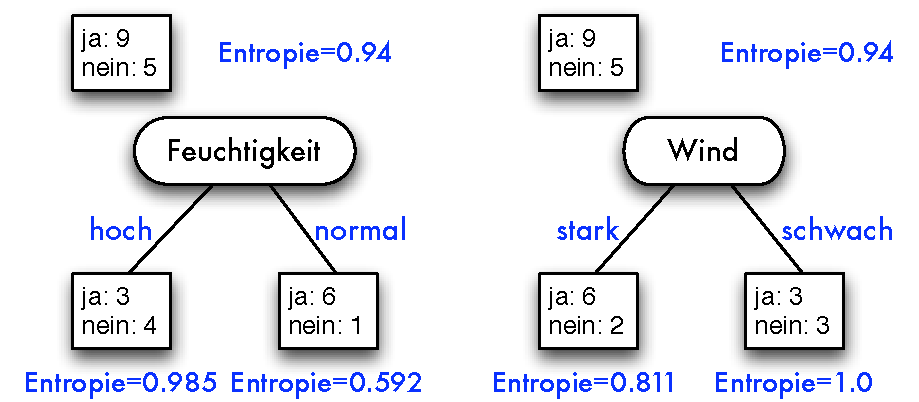
\includegraphics[scale=.5]{fig7/gain-beispiel.pdf}
\end{center}

\begin{eqnarray*}
\textit{gain}(T, \textit{Feuchtigkeit}) &=& 0.94 - (7/14) \cdot 0.985 -
(7/14) \cdot 0.592 \\
 &=& 0.151 \\
\textit{gain}(T, \textit{Wind}) &=& 0.94 - (8/14) \cdot 0.811 -
(6/14) \cdot 1.0 \\
&=& 0.048
\end{eqnarray*}
\end{frame}

%---------------------------------------------------------------------

\begin{frame}
\frametitle{Informationsgewinn: Gain-Ratio}

\begin{eqnarray*}
\textit{gain-ratio}(T,A) &=&
\frac{\textit{gain}(T,A)}{\textit{split-info}(T,A)} \\
\textit{split-info}(T,A)&=&-\sum_{i=1}^m\frac{|T_i|}{|T|} \log \frac{|T_i|}{|T|}
\end{eqnarray*}

\begin{itemize}
\item Anpassung des Informationsgewinns durch Entropie der
  Partitionierung (Split-Info)
\begin{itemize}
\item Paritionierung mit höherer Entropie (viele kleine Partitionen)
  werden bestraft
\end{itemize}
\item Einsatz in C4.5
\end{itemize}

\end{frame}

%---------------------------------------------------------------------

\begin{frame}
\frametitle{Klassifikationsfehler}

$$
\textit{error}(T) = 1 - \underset{i}{\max} p_i
$$
\begin{itemize}
\item misst Klassifikationsfehler pro Knoten
\item Maximum ($1 - \frac{1}{|C|}$): Gleichverteilung der Klassen über
  alle Datensätze 
\item Minimum ($0.0$): alle Datensätze gehören zu einer Klasse

\end{itemize}

\end{frame}

%---------------------------------------------------------------------

\begin{frame}
\frametitle{Klassifikationsfehler: Beispielberechnung}

\begin{itemize}
\item $C_1 = 0$, $C_2 = 6$
\begin{eqnarray*}
p_{C_1}&=&\frac{0}{6} = 0 \quad p_{C_2}=\frac{6}{6}=1\\
\textit{error}&=&1 - \max (0,1) = 0
\end{eqnarray*}
\item $C_1 = 1$, $C_2 = 5$
\begin{eqnarray*}
p_{C_1}&=&\frac{1}{6} \quad p_{C_2}=\frac{5}{6}\\
\textit{error}&=&1 - \max(\frac{1}{6}, \frac{5}{6}) = 1 - \frac{5}{6} =
\frac{1}{6}  
\end{eqnarray*}
\item $C_1 = 2$, $C_2 = 4$
\begin{eqnarray*}
p_{C_1}&=&\frac{2}{6} \quad p_{C_2}=\frac{4}{6}\\
\textit{error}&=& - \max(\frac{2}{6}, \frac{4}{6}) = 1 - \frac{4}{6} =
\frac{1}{3}  
\end{eqnarray*}
\end{itemize}
\end{frame}

%---------------------------------------------------------------------

\frame{
  \frametitle{Ensemble Learning}

  \begin{itemize}
    \item \hl{Ensemble}: Gruppe von Prädiktoren, z.B. Gruppe von Entscheidungsbaumklassifikatoren
    \item liefert häufig bessere Ergebnisse als einzelne Klassifikatoren (,,Wisdom of the Crowd'')
    \item Beispiel: RandomForest = Ensemble von Entscheidungsbäumen
  \end{itemize}

}

\begin{frame}[fragile]
  \frametitle{RandomForest}

    \begin{itemize}
      \item bei jeder Split-Entscheidung wird nur eine zufällig gewählte Teilmenge der Attribute betrachtet
      \item Konstruktion einer größeren Zahl von Bäumen
      \item für Klassifikation Auswertung mit jedem Baum: am häufigsten gewählte Klasse als Ergebnis
  \end{itemize}

  \begin{minted}{python}
from sklearn.ensemble import RandomForestClassifier 

cf = RandomForestClassifier(n_estimators=100, 
     max_leaf_nodes=20, n_jobs=-1)
cf.fit(train_data_x, train_data_y)
pred = cf.predict(test_data_x)
\end{minted}
\end{frame}

\section{Regression}


\frame{
  \frametitle{Überblick}
  \tableofcontents[currentsection,hidesubsections,firstsection=28]
}

\section{Gütemaße}


\frame{
  \frametitle{Überblick}
  \tableofcontents[currentsection,hidesubsections,firstsection=28]
}

%---------------------------------------------------------------------

\frame{
  \frametitle{Evaluation von Data-Mining-Ergebnissen}

  Ziel: Bewertung der Ergebnisse/Modelle
  \begin{itemize}
    \item Parameterwahl?
    \item Qualität der Eingabedaten?
    \item Auswahl des passenden Verfahrens?
    \item \dots
  \end{itemize}

  Gütemaße und deren Bestimmung abhängig von Data-Mining-Problem
}

%---------------------------------------------------------------------

\frame{
  \frametitle{Gütemaße}

  für deskriptive Verfahren: Evaluation anhand der Analysedaten (Trainingsdaten)
  \begin{itemize}
  \item \hl{Clustering}: Kompaktheit, Silhouettenkoeffizient

\end{itemize}

für prädiktive Modelle (Regression, Klassifikation) anhand von Testdaten (nicht Trainingsdaten)!

\begin{itemize}
  \item (Binäre) \hl{Klassifikation}
  \begin{itemize}
    \item Genauigkeit (Accuracy): Anteil der korrekt klassifizierten Objekte
    \item Wahrheitsmatrix (Form der Kontingenztabelle)
    \item Precision (Genauigkeit): $P = \frac{TP}{TP + FP}$
    \item Recall (Trefferquote): $R = \frac{TP}{TP + FN}$
    \item F$_1$-Maß: harmonisches Mittel aus Precision und Recall $F_1 = 2 \cdot \frac{P \cdot R}{P + R}$ 
  \end{itemize}
\end{itemize} 
}


%---------------------------------------------------------------------

\frame{
  \frametitle{Wahrheitstabelle}

  \begin{center}
    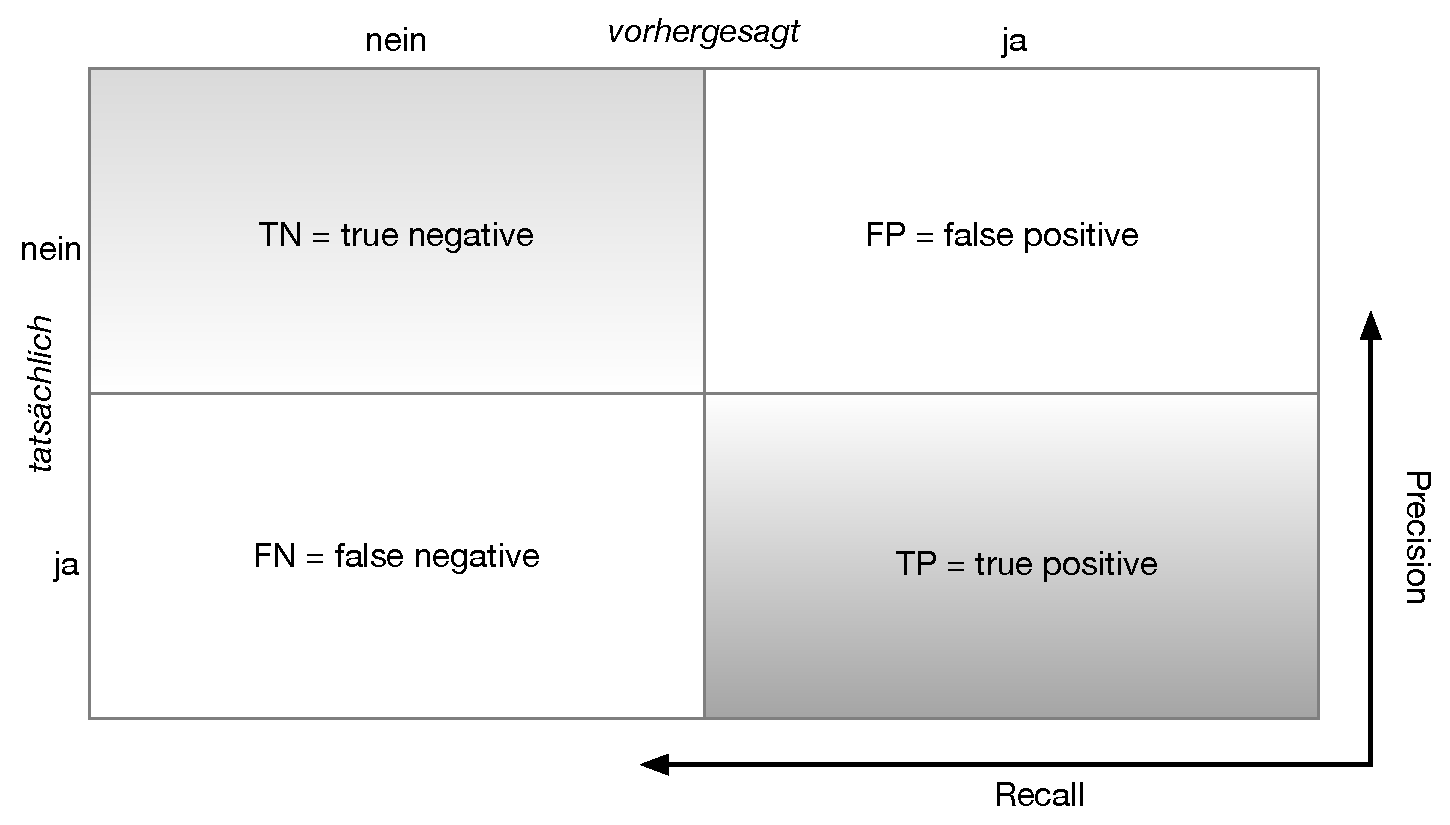
\includegraphics[scale=.45]{fig7/PR-Tradeoff.pdf}
    \end{center}
}

%---------------------------------------------------------------------

\begin{frame}[fragile]
  \frametitle{Precision und Recall mit scikit}

  \begin{minted}{python}
    from sklearn.metrics import precision_score, 
         recall_score, f1_score
    
    precision_score(train_target, train_pred) 
    recall_score(train_target, train_pred) 
    f1_score(train_target, train_pred)
  \end{minted}
\end{frame}

%---------------------------------------------------------------------

\frame{
  \frametitle{Precision/Recall-Tradeoff}

  \begin{itemize}
    \item eigentliches Ziel: hohe Werte für Precision \hl{und} Recall
    \item allerdings nicht möglich 
    \item Schwellwert für Entscheidungen entweder in Richtung Precision \hl{oder} Recall
    \item Priorität für Precision oder Recall abhängig vom Anwendungsfall
  \end{itemize}

  \begin{center}
    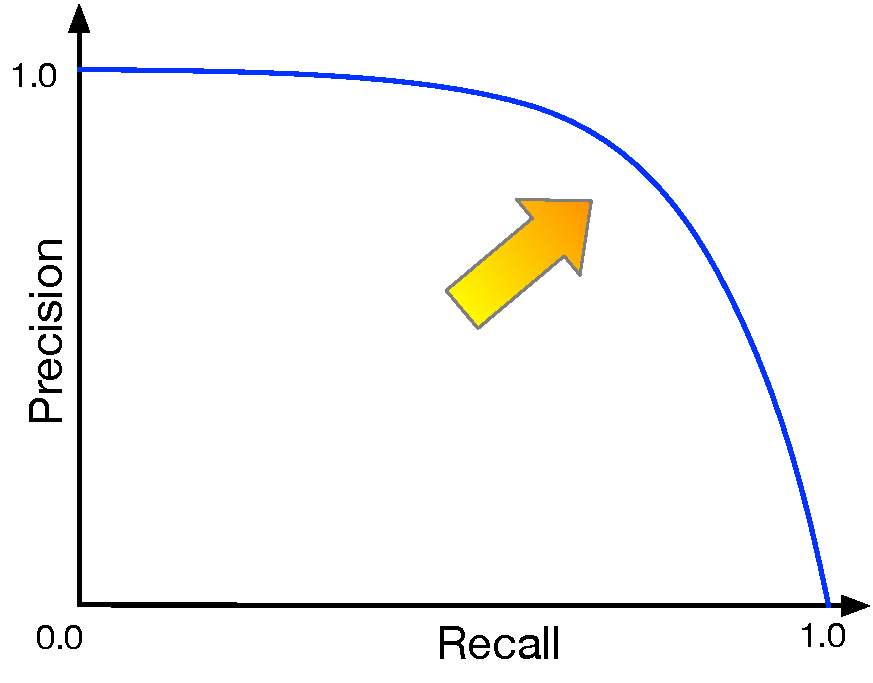
\includegraphics[scale=.3]{fig7/PR-Kurve.pdf}
    \end{center}
}
%---------------------------------------------------------------------
